\title{Model}

{{navbar}}

\subsubsection{Model}

A probabilistic model is a joint distribution $p(x, z)$ of data $x$
and latent variables $z$.
For more details, see the \href{/tutorials/model}{Probability Models tutorial}.
In Edward, we specify models using a simple language of random variables.

\subsubsection{Random Variables}

A random variable $\mathbf{x}$ is an object parameterized by tensors $\theta^*$.
The number of random variables in one object is determined by
the dimension of its parameters.

\begin{lstlisting}[language=Python]
from edward.models import Normal, Exponential

# univariate normal
Normal(mu=tf.constant(0.0), sigma=tf.constant(1.0))
# vector of 5 univariate normals
Normal(mu=tf.constant([0.0]*5), sigma=tf.constant([1.0]*5))
# 2 x 3 matrix of Exponentials
Exponential(lam=tf.ones([2, 3]))
\end{lstlisting}

For multivariate distributions, the multivariate dimension is the
innermost (right-most) dimension of the parameters.

\begin{lstlisting}[language=Python]
from edward.models import Dirichlet, MultivariateNormalFull

# K-dimensional Dirichlet
Dirichlet(alpha=np.array([0.1]*K)
# vector of 5 K-dimensional multivariate normals
MultivariateNormalFull(mu=tf.zeros([5, K]), sigma=...)
# 2 x 5 matrix of K-dimensional multivariate normals
MultivariateNormalFull(mu=tf.zeros([2, 5, K]), sigma=...)
\end{lstlisting}

Random variable objects are equipped with methods such as
\texttt{log_prob()}, $\log p(\mathbf{x}\mid\theta^*)$,
and \texttt{sample()}, $\mathbf{x}^*\sim p(\mathbf{x}\mid\theta^*)$.

Each object wraps a tensor $\mathbf{x}^*$, where
$\mathbf{x}^*\sim p(\mathbf{x}\mid\theta^*)$ is a sample from the
object.

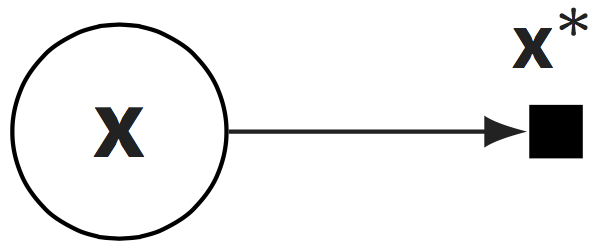
\includegraphics[width=225px]{/images/random_variable.png}

This enables operations on the TensorFlow graph, allowing random
variables to be used in conjunction with other TensorFlow ops. They
operate on $\mathbf{x}^*$.

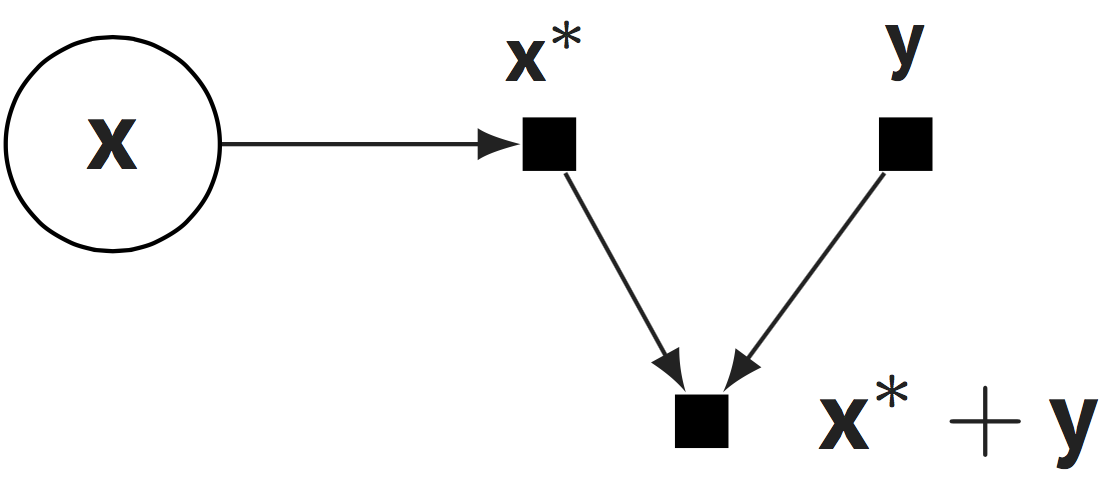
\includegraphics[width=400px]{/images/random_variable_ops.png}

\begin{lstlisting}[language=Python]
from edward.models import Normal

x = Normal(mu=tf.constant([0.0]*10), sigma=tf.constant([1.0]*10))
y = tf.constant(5.0)
x + y, x - y, x * y, x / y
tf.nn.tanh(x * y)
tf.gather(x, 2) # 3rd normal rv in the vector
\end{lstlisting}

We can leverage this construction of random variables to define
models.
For examples of models built in Edward, see the model
\href{/tutorials/}{tutorials}.

\subsubsection{Variational Models}

A variational model defines a distribution over latent variables. It
is a model of the posterior distribution, specifying another
distribution to approximate it.
Edward implements variational models using the same language of random
variables.

We parameterize them with TensorFlow variables so that their
parameters may be trained during inference.

\begin{lstlisting}[language=Python]
from edward.models import Dirichlet, Normal, InverseGamma

qpi_alpha = tf.nn.softplus(tf.Variable(tf.random_normal([K])))
qmu_mu = tf.Variable(tf.random_normal([K * D]))
qmu_sigma = tf.nn.softplus(tf.Variable(tf.random_normal([K * D])))
qsigma_alpha = tf.nn.softplus(tf.Variable(tf.random_normal([K * D])))
qsigma_beta = tf.nn.softplus(tf.Variable(tf.random_normal([K * D])))

qpi = Dirichlet(alpha=qpi_alpha)
qmu = Normal(mu=qmu_mu, sigma=qmu_sigma)
qsigma = InverseGamma(alpha=qsigma_alpha, beta=qsigma_beta)
\end{lstlisting}

\subsubsection{Model Wrappers}

Edward also supports other languages for specifying probability models:
TensorFlow, Python, PyMC3, and Stan.
In each language, a model wrapper is written as a class.

In general, a model wrapper is a class with the structure

\begin{lstlisting}[language=Python]
class Model:
    def __init__(...):
        ...
        self.n_vars = ...

    def log_prob(self, xs, zs):
        log_prior = ...
        log_likelihood = ...
        return log_prior + log_likelihood

model = Model(...)
\end{lstlisting}

The field \texttt{n_vars} denotes the number of latent variables in the
probability model. For example, a model with a Gaussian likelihood with latent
mean and variance would have \texttt{n_vars=2*N} latent variables for
\texttt{N} observations.

The method \texttt{log_prob(xs, zs)} calculates the logarithm of
the joint density $\log p(x,z)$. Here \texttt{xs} can be a single data
point or a batch of data points. Analogously, \texttt{zs} can be a
single set of latent variables, or a batch thereof.

\textbf{TensorFlow.}
Write a class with the method \texttt{log_prob(xs, zs)}. The method defines
the logarithm of a joint density, where \texttt{xs} and \texttt{zs} are Python
dictionaries binding the name of a random variable to
a realization.
Here \texttt{xs} can be a single data
point or a batch of data points, and analogously, \texttt{zs} can be a
single set or multiple sets of latent variables.
Here is an example:

\begin{lstlisting}[language=Python]
import tensorflow as tf
from edward.stats import bernoulli, beta

class BetaBernoulli:
  """p(x, p) = Bernoulli(x | p) * Beta(p | 1, 1)"""
  def log_prob(self, xs, zs):
    log_prior = beta.logpdf(zs['p'], a=1.0, b=1.0)
    log_lik = tf.reduce_sum(bernoulli.logpmf(xs['x'], p=zs['p']))
    return log_lik + log_prior

model = BetaBernoulli()
\end{lstlisting}

\texttt{BetaBernoulli} defines a log joint density with a Bernoulli
likelihood (for an unspecified number of data points) and a Beta prior
on the Bernoulli's success probability.
\texttt{xs} is a dictionary with string \texttt{x} binded to a vector of
observations. \texttt{zs} is a dictionary with string \texttt{z} binded to a
sample from the one-dimensional Beta latent variable.

Here is a
\href{https://github.com/blei-lab/edward/blob/master/examples/tf_beta_bernoulli.py}
{toy script}
that uses this model. The model class can be more complicated,
containing fields or other methods required for other functionality in
Edward. See the section below for more details.

\textbf{Python.}
Write a class that inherits from \texttt{PythonModel} and with the method
\texttt{_py_log_prob(xs, zs)}. The method defines the logarithm of a joint
density with the same concept as in a TensorFlow model, but where
\texttt{xs} and \texttt{zs} now use NumPy arrays rather than TensorFlow tensors.
Here is an example:

\begin{lstlisting}[language=Python]
import numpy as np
from edward.models import PythonModel
from scipy.stats import bernoulli, beta

class BetaBernoulli(PythonModel):
  """p(x, p) = Bernoulli(x | p) * Beta(p | 1, 1)"""
  def _py_log_prob(self, xs, zs):
    log_prior = beta.logpdf(zs['p'], a=1.0, b=1.0)
    log_lik = np.sum(bernoulli.logpmf(xs['x'], p=zs['p']))
    return log_lik + log_prior

  model = BetaBernoulli()
\end{lstlisting}

Here is a
\href{https://github.com/blei-lab/edward/blob/master/examples/np_beta_bernoulli.py}
{toy script}
that uses this model.

\textbf{Stan.}
Write a Stan program in the form of a file or string. Then
call it with \texttt{StanModel(file=file)} or
\texttt{StanModel(model_code=model_code)}. Here is an example:

\begin{lstlisting}[language=Python]
from edward.models import StanModel

model_code = """
  data {
    int<lower=0> N;
    int<lower=0,upper=1> x[N];
  }
  parameters {
    real<lower=0,upper=1> p;
  }
  model {
    p ~ beta(1.0, 1.0);
    for (n in 1:N)
    x[n] ~ bernoulli(p);
  }
"""
model = StanModel(model_code=model_code)
\end{lstlisting}

During inference the latent variable string matches the name of the
parameters from the parameter block. Analogously, the data's string
matches the name of the data from the data block.

\begin{lstlisting}[language=Python]
qp = Beta(...)
data = {'N': 10, 'x': [0, 1, 0, 0, 0, 0, 0, 0, 0, 1]}
inference = Inference({'p': qp}, data, model)
\end{lstlisting}

Here is a
\href{https://github.com/blei-lab/edward/blob/master/examples/stan_beta_bernoulli.py}
{toy script}
that uses this model. Stan programs are convenient as
\href{https://github.com/stan-dev/example-models/wiki}
{there are many online examples},
although they are limited to probability models with differentiable
latent variables. \texttt{StanModel} objects also contain no structure about
the model besides how to calculate its joint density.

\textbf{PyMC3.}
Write a PyMC3 model whose observed values are Theano shared variables,
and whose latent variables use \texttt{transform=None} to keep them on their
original (constrained) domain.
The values in the Theano shared variables can be plugged at a later
time. Here is an example:

\begin{lstlisting}[language=Python]
import numpy as np
import pymc3 as pm
import theano
from edward.models import PyMC3Model

x_obs = theano.shared(np.zeros(1))
with pm.Model() as pm_model:
  p = pm.Beta('p', 1, 1, transform=None)
  x = pm.Bernoulli('x', p, observed=x_obs)

model = PyMC3Model(pm_model)
\end{lstlisting}

During inference the latent variable string matches the name of the
model's latent variables; the data's string matches the Theano shared
variables.

\begin{lstlisting}[language=Python]
qp = Beta(...)
data = {x_obs: np.array([0, 1, 0, 0, 0, 0, 0, 0, 0, 1])}
inference = Inference({'p': qp}, data, model)
\end{lstlisting}

Here is a
\href{https://github.com/blei-lab/edward/blob/master/examples/pymc3_beta_bernoulli.py}
{toy script}
that uses this model. PyMC3 can be used to define models with both
differentiable latent variables and non-differentiable (e.g., discrete)
latent variables. \texttt{PyMC3Model} objects contain no structure about the
model besides how to calculate its joint density.

For modeling convenience, we recommend using the modeling language that
you are most familiar with. For efficiency, we recommend using
TensorFlow, as Edward uses TensorFlow as the computational backend.
Internally, other languages are wrapped in TensorFlow so their
computation represents a single node in the graph (making it difficult
to tease apart and thus distribute their computation).

{{autogenerated}}

\subsubsection{Model Wrapper API}

This outlines the current spec for all methods in the model object.
It includes all modeling languages, where certain methods are
implemented by wrapping around other methods. For example, by a Python
model builds a \texttt{_py_log_prob()} method and inherits from
\texttt{PythonModel}; \texttt{PythonModel} implements \texttt{log_prob()} by wrapping
around \texttt{_py_log_prob()} as a TensorFlow operation.

\begin{lstlisting}[language=Python]
class Model:
  def log_prob(self, xs, zs):
    """
    Used in: (most) inference.

    Parameters
    ----------
    xs : dict of str to tf.Tensor
      Data dictionary. Each key names a data structure used in the
      model (str), and its value is the corresponding corresponding
      realization (tf.Tensor).
    zs : dict of str to tf.Tensor
      Latent variable dictionary. Each key names a latent variable
      used in the model (str), and its value is the corresponding
      realization (tf.Tensor).

    Returns
    -------
    tf.Tensor
      Scalar, the log joint density log p(xs, zs).
    """
    pass

  def log_lik(self, xs, zs):
    """
    Used in: inference with analytic KL.

    Parameters
    ----------
    xs : dict of str to tf.Tensor
      Data dictionary. Each key names a data structure used in the
      model (str), and its value is the corresponding corresponding
      realization (tf.Tensor).
    zs : dict of str to tf.Tensor
      Latent variable dictionary. Each key names a latent variable
      used in the model (str), and its value is the corresponding
      realization (tf.Tensor).

    Returns
    -------
    tf.Tensor
      Scalar, the log-likelihood log p(xs | zs).
    """

  def predict(self, xs, zs):
    """
    Used in: ed.evaluate().

    Parameters
    ----------
    xs : dict of str to tf.Tensor
      Data dictionary. Each key names a data structure used in the
      model (str), and its value is the corresponding corresponding
      realization (tf.Tensor).
    zs : dict of str to tf.Tensor
      Latent variable dictionary. Each key names a latent variable
      used in the model (str), and its value is the corresponding
      realization (tf.Tensor).

    Returns
    -------
    tf.Tensor
      Tensor of predictions, one for each data point. The prediction
      is the likelihood's mean. For example, in supervised learning
      of i.i.d. categorical data, it is a vector of labels.
    """
    pass

  def sample_prior(self):
    """
    Used in: ed.ppc().

    Returns
    -------
    dict of str to tf.Tensor
      Latent variable dictionary. Each key names a latent variable
      used in the model (str), and its value is the corresponding
      realization (tf.Tensor).
    """
    pass

  def sample_likelihood(self, zs):
    """
    Used in: ed.ppc().

    Parameters
    ----------
    zs : dict of str to tf.Tensor
      Latent variable dictionary. Each key names a latent variable
      used in the model (str), and its value is the corresponding
      realization (tf.Tensor).

    Returns
    -------
    dict of str to tf.Tensor
      Data dictionary. It is a replicated data set, where each key
      and value matches the same type as any observed data set that
      the model aims to capture.
    """
    pass
\end{lstlisting}
